\documentclass{bachelor_report}

% Додаткові пакети вносіть у цей файл
\input{01_packages}
\addbibresource{../BIB/Resources.bib}

% Додаткові визначення та перевизначення команд вносіть у цей файл
\input{02_redefinitions}

% Відомості про автора роботи
\input{03_data}

% Починаємо верстку документа
\begin{document}

\setfontsize{14}

% Створюємо титульну сторінку
\input{../CHAPTERS/a1_title}

%% Створюємо зміст    % -- розкоментуйте, якщо зміст вам потрібен
%\pagenumbering{gobble}
\tableofcontents
\cleardoublepage
%\pagenumbering{arabic}

\setcounter{page}{2}    %!!! -- продумати, як автоматизувати номер сторінки

%% Якщо ви використовуєте зміст, то прослідкуйте, щоб номер сторінки 
%% співпадав із справжнім!

% Створюємо перелік умовних позначень, скорочень і термінів
% Якщо цей розділ вам не потрібен, просто закоментуйте два наступних рядка
% \shortings
% \input{../CHAPTERS/a2_shortings}

% Створюємо вступ
\intro
\input{../CHAPTERS/a3_introduction}

% Додаємо глави
% Якщо ваша робота містить менше або більше глав - модифікуйте наступні 
% рядки відповідним чином
\input{../CHAPTERS/c1_chapter_01}
\input{../CHAPTERS/c2_chapter_02}
\chapter{Способи розділення секрету за допомогою асиметричних алгоритмів}
\label{chap:review3}  %% відмічайте кожен розділ певною міткою -- на неї наприкінці необхідно посилатись

\section{Розділення секрету RSA}

\textbf{Розділення секрету RSA} --- це метод розподілу секрету між групою учасників, який відбувається наступним чином:

\begin{enumerate}
    \item Секрет шифрується за допомогою відкритого ключа RSA кожного учасника;
    \item Зашифровані частини секрету передаються відповідним учасникам.
\end{enumerate}

\vspace{0.5cm}
\textbf{Відновлення ж секрету RSA} відбувається наступним чином:

\begin{enumerate}
    \item Кожен учасник розшифровує свою частину секрету за допомогою свого закритого ключа;
    \item Розшифровані частини секрету потім об’єднуються для відновлення оригінального секрету.
\end{enumerate}

\vspace{0.5cm}
Головними перевагами алгоритму RSA є безпека: секрет не може бути відновлений без приватних ключів учасників та гнучкість: поріг відновлення може бути встановлений таким чином, що для відновлення секрету необхідна певна кількість учасників.

Але при цьому алгоритм RSA є нестійким до атак зловмисників, які мають доступ до відкритих ключів учасників та нестійким до квантових атак.

\section{Розділення секрету ECC}

\textbf{Розділення секрету ECC (Elliptic Curve Cryptography)} --- це метод розподілу секрету між групою учасників, який відбувається наступним чином:

\begin{enumerate}
    \item Секрет перетворюється на точку на еліптичній кривій;
    \item Ця точка потім розбивається на n частин, по одній для кожного учасника;
    \item Кожна частина потім шифрується за допомогою відкритого ключа ECC відповідного учасника;
    \item Зашифровані частини секрету передаються відповідним учасникам.
\end{enumerate}

\vspace{0.5cm}
\textbf{Відновлення ж секрету ECC} відбувається наступним чином:

\begin{enumerate}
    \item Кожен учасник розшифровує свою частину секрету за допомогою свого закритого ключа;
    \item Розшифровані частини секрету потім об’єднуються для відновлення оригінальної точки на еліптичній кривій;
    \item Секрет після витягується з цієї точки.
\end{enumerate}

\vspace{0.5cm}
Головними перевагами алгоритму ECC є безпека: якщо приватні ключі учасників є безпечними та стійкість до квантових атак.

Але при цьому алгоритм ECC -- не стійкий до атак зловмисників, які мають доступ до відкритих ключів учасників і складніший у розумінні та реалізації за розділення секрету RSA.

\section{Схема Shamir's Secret Sharing}
\textbf{Схема Shamir's Secret Sharing} --- це алгоритм, вперше запропонований у 1979 році відомим ізраїльським криптографом Аді Шаміром. Він дозволяє розбивати інформацію на багато частин, при цьому вимагаючи лише частину цих частин для відновлення початкового секрету.

Це означає, що замість того, щоб вимагати всіх частин для відновлення початкового секрету, схема Шаміра вимагає мінімальної кількості частин -- цей мінімум називається \textit{порогом}.

\textbf{Розділення секрету Шаміра} --- це метод розподілу секрету між групою учасників, який відбувається наступним чином:

\begin{enumerate}
    \item Секрет ділиться на $n$ частин, де $n$ -- це кількість учасників;
    \item Кожному учаснику надається поліноміальна частка ступеня $m-1$, де $m$ -- це поріг відновлення.
\end{enumerate}

Для того, щоб відновити секрет, необхідно досягти певного порогу. Якщо є щось менше, ніж поріг, секрет не може бути відновлений, таким чином роблячи розділення секрету за Шаміром захищеним від супротивника -- зловмисника, який має необмежену обчислювальну потужність.

\vspace{0.5cm}
Однією з переваг алгоритму Шаміра є те, що він є гнучким і розширюваним -- тобто власник секрету може додавати, змінювати або видаляти частки в будь-який час, якщо захоче, без зміни початкового секрету. А також він стійкий до атак зловмисників, які мають доступ до відкритих ключів учасників, і ще стійкий до квантових атак, оскільки ґрунтується на інтерполяції многочленів, яка є проблемою, яка, є складною для квантових комп’ютерів.

Але при цьому алгоритм Шаміра менш ефективний, ніж RSA або ECC, та крім цього -- необхідно зберігати додаткову інформацію (наприклад, коефіцієнти полінома), щоб відновити секрет.

\newpage
\section{Порівняння ефективності алгоритмів за обраним критерієм}

Для порівняння ефективності алгоритмів було взято в якості критерію -- кількість обчислювальних операцій, необхідних для розподілу та відновлення секрету, де: 
\vspace{0.25cm}
\begin{itemize}
    \item n - кількість учасників
    \item m - поріг відновлення.
\end{itemize}

\begin{table}[ht]
\centering
\scalebox{1.25} {
\begin{tabular}{|c|c|c|}
\toprule
        \textbf{Алгоритм} & \textbf{Розподіл} & \textbf{Відновлення} \\ \midrule
	RSA & $O(n^2)$ & $O(m^2)$ \\ \cmidrule{1-3}
	ECC & $O(n^2)$ & $O(n)$ \\ \cmidrule{1-3}
        Схема Шаміра & $O(n^3)$ & $O(n^2)$ \\ \bottomrule
\end{tabular}}
\end{table}

Також було проведено загальне порівняння алгоритмів:

\begin{figure}[ht]
        \centering
        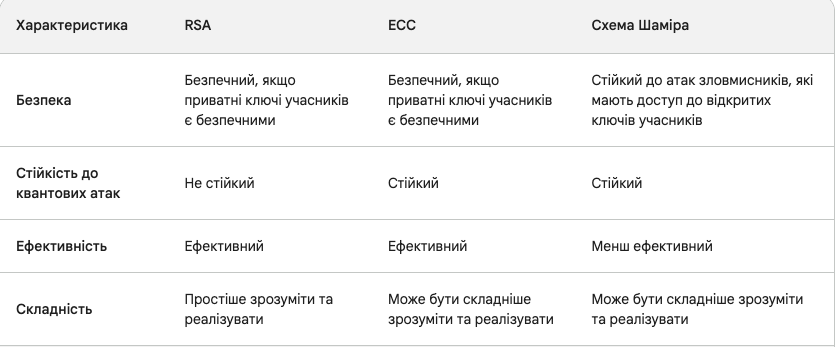
\includegraphics[scale=0.6]{IMAGES/compareTable.png}
        \caption{Загальне порівняння}
        \label{fig_compareTable}
\end{figure}

% \newpage
\chapconclude{\ref{chap:review3}}
В даному розділі було розглянуто та порівняно різні способи розділення секрету за допомогою асиметричних алгоритмів. Також визначено, що розділення секрету не може гарантувати абсолютну безпеку секрету, але може значно ускладнити його розкриття зловмисниками. Використання методів розділення секрету може значно підвищити безпеку та конфіденційність інформації.\par
В результаті порівняння маємо наступне:
\begin{itemize} [label={$\bullet$}]
    \item RSA має найгіршу ефективність при відновленні секрету, але вона проста у реалізації + використовує експоненційні операції, які є обчислювально складними;
    \item ECC має кращу ефективність при відновленні секрету, але вона складніша у реалізації + використовує експоненційні операції, які є обчислювально складними;
    \item Схема Шаміра має найгіршу ефективність при розподілі секрету, але вона стійка до атак зловмисників, які мають доступ до відкритих ключів учасників + використовує інтерполяцію многочленів, яка є менш обчислювально складною.
\end{itemize}

% Створюємо висновки
\conclusions
\input{../CHAPTERS/w1_conclusions}

% Додаємо бібліографію
% Якщо ви володієте магією bibtex-у, використовуйте її та модифікуйте файл 
% з бібліографією відповідним чином
\bibliographylist
\printbibliography[heading=none]
% \input{BIB/RESOURCES.bib}

% Створюємо додатки (дивись у файли додатків для необхідних пояснень)
% Якщо ви маєте меншу або більшу кількість додатків, модифікуйте наступні 
% рядки відповідним чином
% Якщо ви не маєте додатків, просто закоментуйте наступні рядки
%\input{../CHAPTERS/z1_appendix_A}


% Нарешті
\end{document}